\documentclass[7pt,a4paper]{article}
\usepackage{clrscode}
\usepackage[conEntregas]{caratulaTP1}
\usepackage[spanish]{babel} % para que comandos como \today den el resultado en castellano
\usepackage{a4wide} % márgenes un poco más anchos que lo usual
\usepackage[T1]{fontenc}
\usepackage{textcomp}
\usepackage{graphicx}
\usepackage[utf8]{inputenc} 
\usepackage{pdfpages}
\usepackage{amsmath}
\usepackage{vmargin}
\setpapersize{A4}
\setmargins{0.5cm}       % margen izquierdo
{0.5cm}                        % margen superior
{19.0cm}                      % anchura del texto
{26.42cm}                    % altura del texto
{3pt}                           % altura de los encabezados
{1cm}                           % espacio entre el texto y los encabezados
{0pt}                             % altura del pie de página
{1cm}                           % espacio entre el texto y el pie de página
\usepackage{ftnxtra}
\usepackage{listings}
\usepackage{xcolor}
\lstset { %
    language=C++,
    backgroundcolor=\color{black!5}, % set backgroundcolor
    basicstyle=\tiny,% basic font setting
    breaklines=true,
}

\begin{document}
\titulo{Trabajo Práctico 1}
\subtitulo{Eligiendo justito}

\fecha{\today}

\materia{Algoritmos y Estructura de Datos III}

\integrante{Buceta, Diego}{001/17}{diegobuceta35@gmail.com}
% Pongan cuantos integrantes quieran

\maketitle

\newpage
%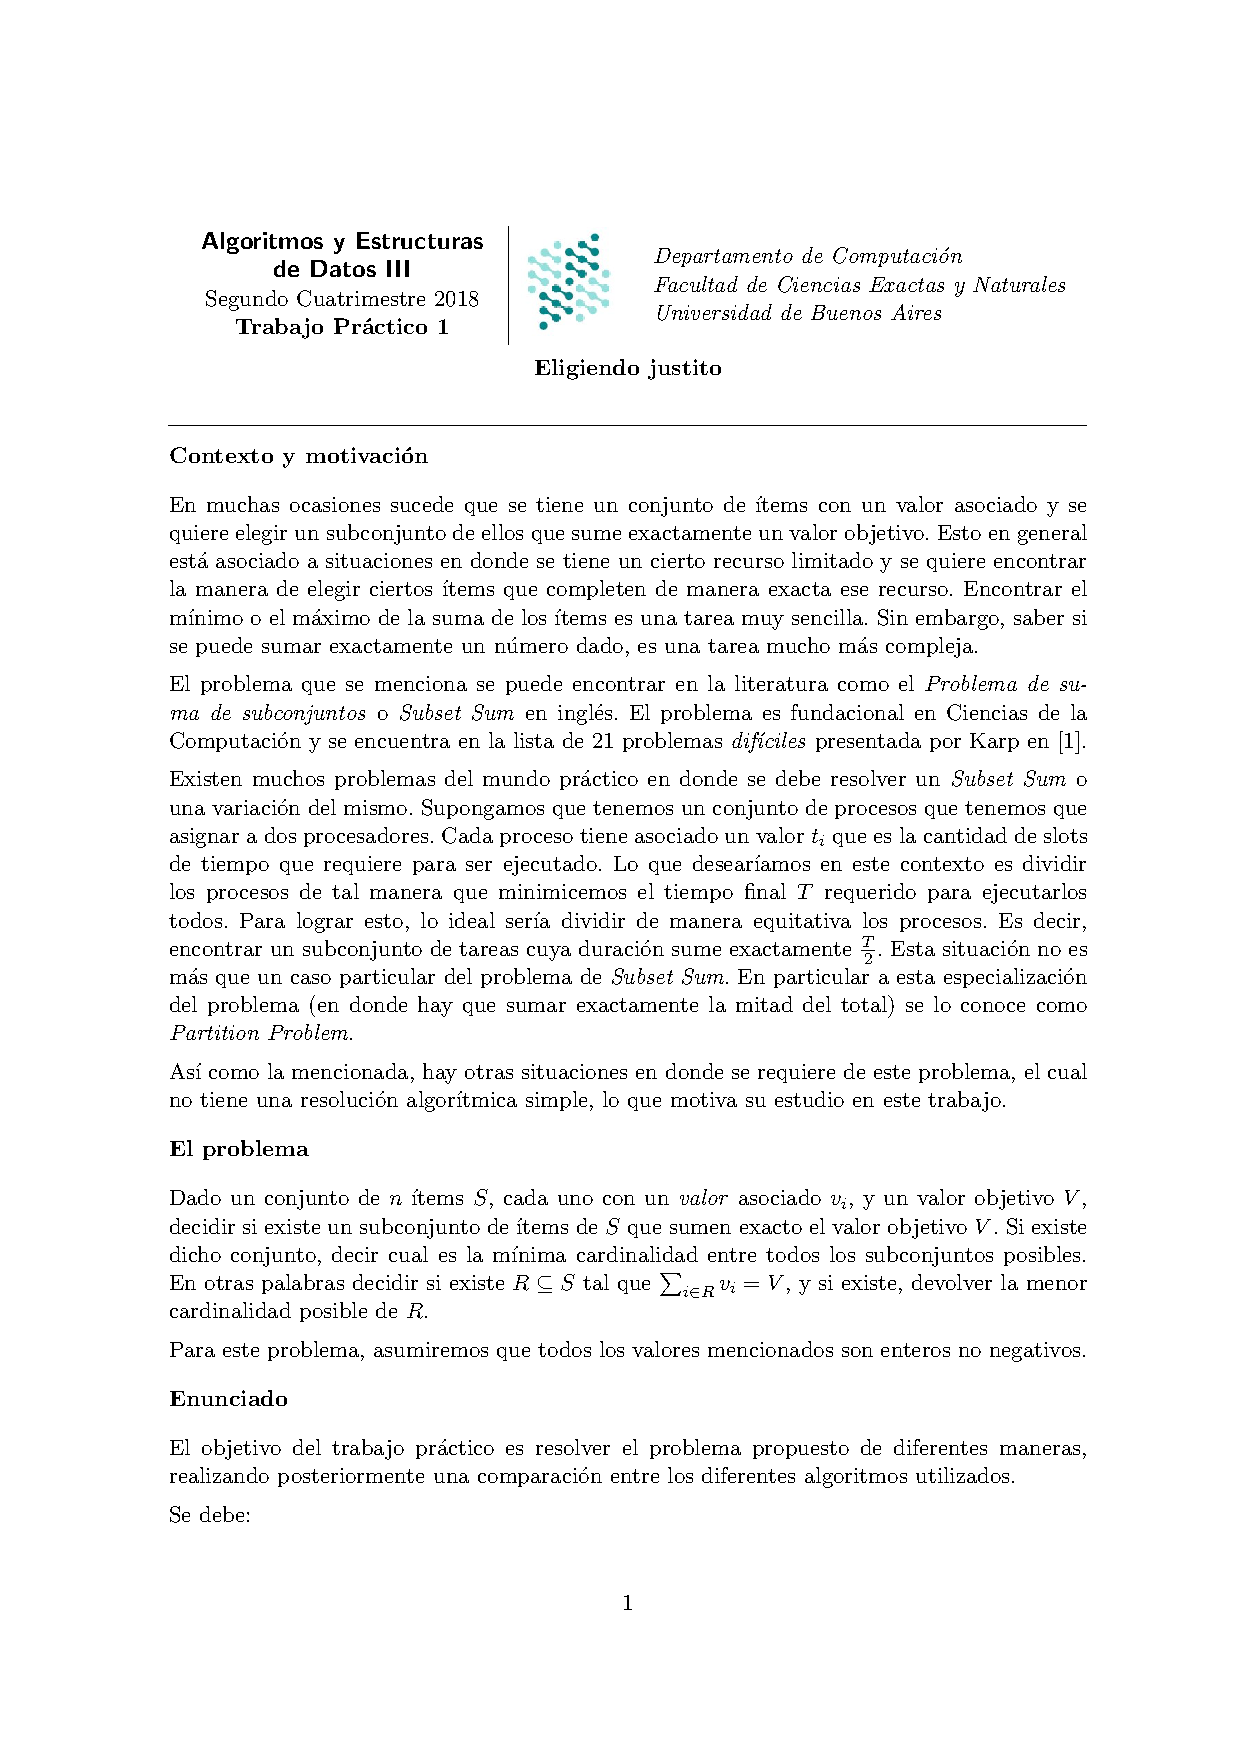
\includepdf[pages={1,2}]{tp1.pdf}

\section{Introducción}
\subsection{El problema y sus análisis}
\begin{verse}
	El subset sum problem o problema de la suma de conjunto es un problema muy conocido dentro de las ciencias de la computación y matemática por ser un objeto de estudio dentro de la clase  NP-problem \footnote{Problemas de decisión y optimización donde se busca encontrar si existe solución o si existe una mejor que la conocida}, se destaca por su facilidad para describirlo y gran dificultad para resolverlo. Los algoritmos más conocidos que pueden resolverlo tienen una complejidad temporal exponencial y esto se traduce en imposibilidad de resolverlo en casos donde la cantidad de elementos sea grande. \\
Además de las diferentes versiones de este problema \footnote{Problema de la carga de la mochila; Problema de selección de conjuntos de un conjunto, etc} existen usos muy diversificados en el ámbito cotidiano y científico. No solo sirve como fuente de nuevas investigaciones en el campo de la teoría de complejidad sino también en ramas como la criptografía, programación genética, etc$[3][4]$. %Imaginemos un algoritmo que resuelva problemas a modo de entrenamiento, problemas de tamaños variados y que en muchos casos es necesario clasificar las diferentes soluciones. En los algoritmos genéticos se suele desarrollar un algoritmo que funcione o se comporte como un gen y evaluarlo en consecuencia. Existen casos en los que el output no tienen una correlación real con un gen y es necesario técnicas de apartado o filtrado obtener los más aproximados, y una de ellas está fuertemente relacionada con el Subset Sum Problem.\\

\bigskip
	Definición: Dado C conjunto de enteros no negativos y V entero no negativo se desea saber si existe un s $\subseteq$ S tal que $\sum_{r \in R}r$ = V, y si existe que tenga la mínima cardinalidad.
	
	\paragraph{Intuición} 	Una de las primeras aproximaciones para buscar una solución puede ser la de formar todos los conjuntos posibles con los elementos de S y analizar si alguno suma V. Por un lado, este algoritmo asegura que si existe solución se va a encontrar; por el otro lado y como contrapartida de lo anterior, si no existe solución o S es muy grande la cantidad de pruebas que son necesarias superará las capacidades de cómputo actuales. %En la actualidad hay diversas ramas que se encuentran con estas dificultades, y la manera en que se suelen evitar es utilizando aproximaciones para el problema y no algoritmos exactos$[5]$. reducir esto tampoco tiene sentido la suposición de determinadas características de S, como el orden de sus elementos, dado que siempre se verificarán todos los subconjuntos.
	%Un tamaño de S mayor a 80 con este tipo de técnicas significaría un desafío para las capacidades de los procesadores actuales. Si bien las instrucciones por segundo que pueden realizar dependen de muchos factores como cantidad de instrucciones por ciclo del reloj de procesador, cómo interactúa un determinada software con el procesador, la memoria, núcleos del procesador, factores externos, etc, solo un vistazo a la siguiente tabla evidencia aún más el problema. 	\bigskip
		 %El problema crece exponencialmente respecto al crecimiento de S y si se tiene en cuenta que las procesadores de computadoras personales en promedio pueden tener alrededor de 700GFlops \footnote{Billión de operaciones flotantes por segundo, medida que se utiliza para medir perfomances en los campos científicos computación}, lo que establece una proporción aproximada entre los calcúlos de cantidad de subconjuntos y capacidad de operaciones del procesador de 1 $\approx$ 2000000 operaciones.	\bigskip
	
%\begin{center}
%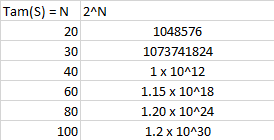
\includegraphics[scale=.7]{tabla.png}
%\end{center}
	\paragraph{Otras formas} Los análisis previos arrojan suficientes razones como para ahondar en otras soluciones.
	\bigskip
	
		Una algoritmo publicado por Horowitz Ellis y Sahni Sartaj $[6][7]$ consiste en dividir los n elementos en dos conjuntos separados, cada uno con $\frac{n}{2}$ elementos. Para cada uno de los conjuntos se almacenan en dos listas la suma de los posibles subconjuntos junto con su cardinal. Posteriormente se utiliza algún algoritmo de comparaciones para ordenarlas, L$_{1}$ en orden decreciente y L$_{2}$ creciente, lo que suma una complejidad temporal de 2 $\cdot$ O($2^{\frac{n}{2}} \cdot \frac{n}{2}$). Con las dos listas ordenadas, la idea principal es tomar un elemento de cada lista y compararlo con V. Por un lado se toma el elemento más grande (primero )de L$_{1}$ y el más chico (primero )de L$_{2}$. Entonces: 

	\begin{itemize}
	\item Si la suma supera a V: El algoritmo avanza un elemento en L$_{1}$
	\item Si la suma es menor a V: El algoritmo avanza un elementom en L$_{2}$
	\item Si la suma coincide con V: se muestra la solución.
	\end{itemize}
	%La complejidad temporal sería del orden O($2^{\frac{n}{2}} \cdot n $). Si se tiene en cuenta el crecimiento exponencial reltivo a n, conseguir una solución que reduzca n a $\frac{n}{2}$ no es poca cosa. \\
	
	
%	Otras soluciones proponen encontrar algoritmos pseudo-polinomiales respecto de n en complejidad temporal. Dado que se busca responder a un problema de forma exacta, las complejidades polinomiales no se pueden esperar.
%	A modo de esclarecer, establezcamos qué es uno y otro.\footnote{Definiciones tomadas del libro Thomas Cormen, Introduction Algorithms. Capítulo NP-Problems, página 1048.}
%	Por un lado, la complejidad de diferentes algoritmos puede cambiar radicalmente en función de los parámetros que depende, y en diferentes circustancias o bajo determinadas suposiciones pueden tomarse los que se consideren apropiados.\\
%	Por ejemplo, en un algoritmo de ordenamiento de comparacion1es, la mejor complejidad que se puede tomar es O($log_2 n \cdot n$), con n cantidad de números. Sin embargo, si se sabe que los números están acotados por una constante K, podría aplicarse un counting-sort y reducir la complejidad a O(K + n) $\approx $ O(n). En caso de que k esté acotado por n, el algoritmo sería O(2n), o sea lineal.\\
%	Este análisis permite ver que incluso definiendo la complejidad en función del tamaño de la entrada los resultados pueden varían. \\
%	La definición formal de complejidad algorítmica temporal habla de que se mide en función del tiempo requerido en función del tamaño de la entrada.
%	Trabajando con enteros de una cantidad acotada de k bits, podemos establecer que la complejidad de nuestra entrada sería O(k $\cdot$ n) $\approx$ O(n).\\
%	\subparagraph{Definición:}	
%	Un problema tiene complejidad en tiempo polinomial si existe un algoritmo que lo resuelva en O($n^{m}$), donde m es constante. Si el problema se puede resolver se lo denomina fácil o tratable y en caso contrario difícil o no tratable. Imaginar esto no resulta complicado dado que m podría ser un número grande como 100 para un exponente y si bien $2^{100}$ sigue siendo polinomial la realidad es que ahora sería un problema difícil. \\ Por esto, existen muchas consideraciones para las complejidades dentro de lo polinomial: pseudopolinomial, quasipolinomial, subpolinomial, etc, pero sólo vamos a adentrarnos en un caso más para nuestro análisis.\\
%	Cuando se habla de algoritmo pseudo-polimial significa que es polinomial respecto del máximo valor númerico de la entrada, y no del tamaño de la entrada.
%	O sea que si podríamos suponer que existe una cota para los valores de S, digamos que están acotados por k = $n^{2}$ y hay n = 100, entonces ninguno superará a 10000. Entonces el algoritmo sería polinomial en esa cantidad fija, digamos W y como es acotada por un polinomio de n, digamos $n^{m}$ entonces el algoritmo es polinomial O($n^{m \cdot W}$).

	%Un breve análisis de este problema permitió profundizar acerca de las soluciones encontradas hasta el momento, las diferentes técnicas y formas de expresar sus dificultades utilizadas, y por qué es un objeto tan importante dentro de las ciencias de la matemática y computación este tipo de problemas considerados los NP-P problems.
\end{verse}
\section{Algoritos presentados}
En este trabajo presentaremos diferentes algoritmos con los que buscaremos experimentar y encontrar los contextos en los cuales sería beneficioso la aplicación de alguno de ellos.
\subsection{Fuerza Bruta}
Esta forma de resolver el problema está fuertemente relacionada con las primeras técnicas que surgieron para el problema de la suma de subconjuntos. Lo primero que debe hacerse es definir un dominio de posibles soluciones del problema, y posteriormente describir un algoritmo que permita alcanzarlas a todas. \\

	En nuestro problema, vamos a definir nuestro espectro de posibles soluciones al conjunto de partes del conjunto inicial, S. Este conjunto estará formado por todos los posibles subconjuntos que se puedan tomar con elementos de S. Dado que cada elemento tiene dos opciones, estar o no en un determinado subconjunto, las opciones entonces son: 2 $\cdot$ 2 $\cdot$ 2  $\cdots$ 2 = $2^{n}$
%Por la propia definición, es trivial que si llegará a existir un conjunto R contenido en S y que la sumatoria de sus elementos sea V lo vamos a poder encontrar. Además, almacenando como nueva solución sí y solo sí la encontrada es mejor que la anterior o si no existía,se encontraría en particular la que tenga menos elementos.
\subsection{Algoritmo}

% Updates to \Then and \Else
\renewcommand{\Then}{%
  \textbf{then}\stepcounter{indent} }
\renewcommand{\Else}{%
  \kill\addtocounter{indent}{-1}%
  \liprint\textbf{else}\>\>\stepcounter{indent}}
\renewcommand{\Until}{%
  \addtocounter{indent}{-1}%
  \kill\liprint\textbf{until} }

\begin{codebox}
  \Procname{$\proc{FuerzaBruta}(Conjunto(enteros):C,entero: V)$}
  \li $i \gets 0$
  \li $P \gets generarPartes(C)$
  \li $sol \gets -1$
  \li $n \gets Tam(C)$
  \li \Repeat
  \li   $suma \gets sumaElementos(P, i)$
  \li   $card \gets cantElementos(P, i)$
  \li   \If $suma == V$ \Then
  \li 	\If $sol == -1$ \Then
  \li     $sol \gets card$
  \li 	\Else 
  \li 	\If $sol > card$ \Then
  \li 	$sol \gets card$
  		\End
        \End
        \End
  \li \Until $i <= 2^{n}$
\end{codebox}

%\paragraph{Detalle}

%	El algoritmo se basa en analizar la suma de elementos de cada uno de los $2^{n}$ subconjuntos que puede formarse y compararlos con V. Si ya existiese una solución sólo la renombraríamos si la actual es mejor, es decir, el subconjunto tiene menos elementos.
%	\\ Los puntos importantes del pseudocódigo están en (2)(6)(7) porque es donde están los pasos {\it no triviales}. \\
\subparagraph{Función: generarPartes} El código fuente del problema genera el conjunto de partes de la siguiente manera: una variable $i$ se mueve entre 0 y $2^{n}$ - 1, y en cada uno de esos valores analiza su representación en bits y además otra variable $j$ se mueve entre 0 y n-1. Es decir, cada vez que i actualiza su valor, j se actualiza n veces. En esas n comparaciones lo que se hace es analizar si el bit jésimo se corresponde un bit marcado en uno de i. Si esto pasa, significa que en el subconjunto iésimo debe estar el elemento j, y así para cada elemento. Esto se hace mediante el corrimiento de bits en O(1) que ofrece $C++$.
\subparagraph{Función: sumaElementos y cantElementos} Dado un conjunto de conjuntos y un valor,  una retorna la suma y la otra el cardinal del subconjunto i-ésimo. A modo de una mejor visualización de las ideas del algoritmo estas funciones cumplen un objetivo simbólico y no tienen una correspondencia simétrica con el código, en caso de plasmar este pseudocódigo en un lenguaje, simplemente cambiará la complejidad espacial debido a que habría $2^{n}$ subconjuntos almacenados.

\subsubsection{Complejidad}
Desde el punto de vista de complejidad, si se define en función del tamaño de entrada, y tomando n como el tamaño de S, nuestro algoritmo será $\theta$(n $\cdot$ 2$^{n}$), porque se recorrerá cada subconjunto del conjunto de partes de S y para cada uno revisará cuáles de los n elementos de S están en ese subconjunto.\\
%Si se definiera en función de m = $\max C$ y si m = $2^{n}$, la complejidad seria O(m $\cdot \log_{2}{m}$ ), valor que en la práctica se podría considerar lineal (respecto a m), una diferencia demasiado grande con respecto a una complejidad exponencial. Resulta interesante pensar en cómo se verá todo estas variaciones en las experimentaciones de este algoritmo.


\subsubsection{Código Fuente}
\begin{lstlisting}
int bruteforce(vector<int>& c,  long long int valorObjetivo,int &sol,long long int &pasos){
    int n = c.size();
    long long int total = pow(2,n);
    sol=-1;
    for (long long int i=0; i< total; i++) {
        long card=0;
        long sum = 0;
        for (int j=0; j<n; j++){
            pasos++;
            if (i & (1 << j)) { //chequeo si el elem jesimo tiene el bit en 1 (es decir, debe estar en el subconjunto i), si es 0 no esta entonces lo salto.
                card++;
                sum += c[j];
            }

        }
        if(sum == valorObjetivo) {
            if(sol==-1){
                sol = card;
            }else {
                if(sol > card) {
                    sol = card;
                }
            }
        }
    }
    (sol == -1 || sol >= n)? sol = -1:1;
    return sol;
}

\end{lstlisting}

\subsection{Backtracking}
Lo que caracteriza a esta forma de resolver el problema es que vamos a buscar definir situaciones en las que seguir computando la solución no tenga sentido. Esto quiere decir abandonando posibles candidatos a solución por temás de optimalidad o posibilidad de la solución, a esto se lo denomina podas. \\
%Si se modela el Backtracking como un árbol binario[\footnote{Donald Knuth. \it{The Art Of Computer Programming : Fundamentals Algorithms.} Capítulo 2}] puede pensarse que cada nodo representa un nuevo sub-problema o llamada recursiva del problema anterior y puede tener a lo sumo dos llamadas recursivas, es decir, dos hijos. Esto significa que en un árbol balanceado la profundidad será $\log_{2}(2^{n})$ = $n$ y las llamadas recursivas va a estar acotada superiormente por la cantidad de nodo que será:$\approx$ $2^{n}$

%Para nuestro caso en particular, vamos a suponer que nuestro conjunto C viene ordenado. Podemos hacerlo porque en caso de que no venga se lo ordena en $\log_{2}n \cdot n$ con algún algoritmo que como merge-sort, que no afecta la complejidad a la que nos debemos ajustar. La razón de tenerlo ordenado en forma creciente es que vamos a poder establecer cotas de complejidad más fuertes.
\subsubsection{Podas}
\begin{itemize}
	\item 
	Por optimalidad: Si en el proceso de computo de una posible solución, se llegara al caso en que el subconjunto de elementos actual contiene más elementos que la mejor solución encontrada hasta ahora, entonces no se buscará y computará ninguno de los subconjuntos que surjan de tener como los primeros k elementos del subconjunto actual y siendo k el tamaño de éste.
	\item 
	Por factibilidad: Si en el proceso de cómputo de una posible solución, se llegara al caso en que la sumatoria de los elementos del conjunto formado actual supera a V, significa que no tiene sentido probar con a ninguno de los elementos hacia la derecha, porque están ordenados de forma creciente, y ninguno de los conjuntos que surjan de combinar los elementos restantes de S con el conjunto actual van a funcionar.
\end{itemize}

%Breve ejemplo con C = $\{$ 2, 3 , 6$\}$ y valor objetivo V = 5.\\
%Se observan los nodos verdes que son los caminos que se siguen y los rojos los que se podarían
%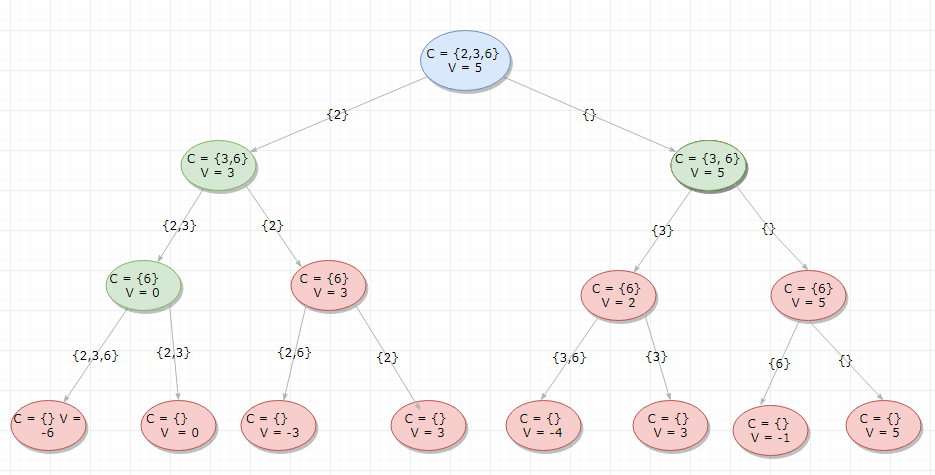
\includegraphics[scale=.7]{grafico_backtracking.png}

La siguiente imagen muestra la idea de las podas. Si tomamos el punto amarillo superior como el inicio de una parte de los posibles caminos del problema total vemos cómo las flechas verdes marcan los caminos que se siguieron por cada nodo y cómo al llegar a puntos \textcolor{red}{problemáticos} las flechas rojas marcan el retroceso y recorrido de otro camino, hasta agotarlos a todos. Los puntos \textcolor{red}{problemáticos} simbolizan otros inicios de conjuntos de caminos que por algún motivo se decide 'podarlos' y no analizarlos en profundidad.

\begin{center}
\includegraphics[scale=.2]{backtrack}
\footnote{Imagen tomada del blog de Steve Pemberton}
\end{center}
\subsubsection{Algoritmo}

\begin{codebox}
  \Procname{$\proc{Backtracking}(Conjunto(enteros):C,entero:sol,entero: V, entero:desde,entero:sumaElem,entero:cantElem)$}
  %\li $sol \gets -1$
  %\li $sumaElementos \gets sumaConj(conjAct)$
\li 	\If $sol = -1$ $or$ $sol !=-1$ $and$ $cantElem < sol$ \Then  
  %\li \If $todavia$ $no$ $se$ $encontro$ $solucion$ $o$ $si$ $se$ $encontro$ $y$ $el$ $conjunto$ $formado$ $actual$ $tiene$ \\ $menos$ $elementos$ \Then 
  \li 	\If $sumaElementos = V $ \Then
  		\li \If $sol = -1$ $or$ $sol > cantElem$ \Then
  			\li	$sol \gets cantElem$
  			\End
  		\End
  \End 
  \li $i \gets desde$
  \li \While  $i <= |C|$ $and$ $sumaElementos <  V $ \li \Do
  \li \If $(sol = -1$ $or$ $sol < cantElem)$ \Then
  %\li $agregar(conjAct, C_{i})$
  
  \li $cantElem \gets cantElem +1$
  
  \li $sumaElementos \gets sumaElementos+C_{i}$
  \li $i \gets i + 1$ 
  \li $Backtracking(C,sol,V,i,sumaElementos,cantElem)$
  %\li $eliminarUltimoElemento(conjAct)$
  \li $cantElem \gets cantElem - 1$
  \li $sumaElementos \gets sumaElementos - C_{i}$
  
  \End
  \End 
\end{codebox}

\subparagraph{Detalle} Como se mencionó anteriormente, suponemos que existe una función auxiliar que llama a esta con los valores de los parámatros bien definidos y C ordenado. La idea del algoritmo es recorrer cada elemento del conjunto de entrada a partir del flag {\it desde}. Mientras no se necesite podar, el algoritmo acumula el valor de los elementos y la cantidad de ellos entre {\it desde} y el final de C. Al mismo tiempo, se recursiona con un C' = C $-$ ${C_{iteracion_actual}}$ y los flags actualizados, o sea, la variable de inicio del subproblema a resolver ahora comenzará en la iteración actual. A {\it sumaElementos} se le descontará el último elemento sumado y {\it cantElem} se reducirá en uno; que es igual a C sin el elemento de la iteración actual. Si se encuentra solución, se almacena en {\it sol}, sin embargo y dado que la diferencia de esta técnica con fuerza bruta es que se trata de apartar candidatos a solución por temas de optimización o factibilidad, el algoritmo termina después de haber intentado analizar todos los posibles subconjuntos del C inicial. \\
Al comienzo, esta función se llama con los flags {\it desde} = 0, {\it sol} = -1, {\it cantElem} = 0 {\it sumaElementos} = 0.
\subsubsection{Complejidad}

Respecto a la complejidad temporal y estableciéndola en función de tamaño de la entrada, $|$S$|$ = n, analicemos cuál sería el peor caso. El peor caso sería que las podas que definimos no funcionen, y eso pasa si el V que se elige supera a la suma de todos los elementos de C. Con un caso así, nunca sería necesario podar soluciones por factibilidad, porque nunca existirá un subconjunto de C que sume más que V si la suma de C no lo suma y por otro lado como no habrá solución, nunca habrá podas por mejor solución.\\
En cada paso, el algoritmo realiza a lo sumo n pasos y la complejidad del algoritmo se puede establecer de forma recursiva con la siguiente funcion:
\begin{align}
 T_{n} = (n-1) T_{n-1} + (n-1) ,
\end{align}

Sea T' lo siguiente y definiendo y T'(0)=0:
\begin{align}
 T'_{n} = T'_{n-1} + n,  n = 1, 2, 3...
 T'(n) = T'(n-1) + n = T'(n-2) + (n-1) + n \\  = T'(n-k) + n-k-1 + n-k-2 + ... + n-1 + n = \sum_{i=1}^{n}i,
 \end{align}
 \begin{verse}
 Por suma de Gauss:
 \end{verse}
 \begin{align}
 = \frac{(n\cdot(n+1))}{2} = \frac{n^{2}}{2} \in O(n^{2})
\end{align}

\begin{verse}
De modo que la complejidad de T' $\in$ O($n^{2}$). Ordenar inicialmente a C no nos modifica la complejidad porque sería simplemente O(T(n)) + O($\log_{2}n \cdot n$) que sigue siendo asintóticamente acotado superiormente por nuestra cota.

Veámos que T'$_{n}$ $\cdot$ (n-1) $\approx$ T$_{n-1}$ $\cdot$ (n-1) + $n^{2}$, que por lo visto antes $\in$ O(n) $\cdot$ O($n^{2}$) $\cdots$ ¿$\in$ O($2^{n} \cdot n$ )?  \\
Sea C constante, vemos si existe un valor $x_{i}$ tal que $\forall$ $x_{j}$ $\geq$ $x_{i}$ a partir del cual valga:
\end{verse}

\begin{align}
n^{3} \leq c \cdot 2^{n} \cdot n, \text{  n $>$ 0}, n^{2} \leq c \cdot 2^{n}
\end{align}
\begin{verse}
Aplicamos función creciente a ambos lados sin cambiar la desigualdad
\end{verse}
\begin{align}
\log_{n} n^{2} \leq c \cdot n, 2 \log_{n}n \leq c \cdot n
\end{align}
Y esto es cierto. Ahora falta ver si O(T$_{n}$) $\in$ O(T$_{n-1}$ $\cdot$ (n-1) + $n^{2}$).\\
Sea K constante, vemos si existe un valor $x_{i}$ tal que $\forall$ $x_{j}$ $\geq$ $x_{i}$ a partir del cual valga:
\begin{align}
	T_{n-1} \cdot (n-1) + n < K (\cdot T'_{n-1} \cdot (n-1) + n^{2})
\end{align}
Si K = 1
\begin{align}
	 n < n^{2}
\end{align}
\\ Entonces el algoritmo de backtracking $\in$ O($2^{n} \cdot n$)


\subsubsection{Código Fuente}
\begin{lstlisting}

int backtracking(vector<int> c,  long long int valorObjetivo, int& sol,long long int &pasos) {
    sol=-1;
    sort(c.begin(),c.end()); //ordenamos de menor a mayor en aprox segun c++ (log |c| * |c|)
    auxBacktracking(c,0,valorObjetivo,sol,0,0,pasos);
    if(sol==-1 || sol >= c.size()) {
        return -1;
    }else{
        return sol;
    }
}

void auxBacktracking(vector<int>& c, int desde,  long long int valorObjetivo, int& sol, long long;  int sumaActual,  long long int cantElem,long long int &pasos){
    if(sol==-1 || (sol != -1 && cantElem < sol)){
        if(cantElem > 0) {
            if(sumaActual == valorObjetivo) {
                if(sol==-1){
                    sol = cantElem;
                }
                else {
                    if(sol > cantElem) {
                        sol = cantElem;
                    }
                }
            }
        }
    }
    for (int i = desde; i < c.size() && sumaActual < valorObjetivo; ++i) {
        pasos++;
        if( sol==-1 || sol!=-1 && sol > cantElem) {
            desde++;
            sumaActual +=c[i];
            cantElem++;
            auxBacktracking(c,desde,valorObjetivo,sol,sumaActual, cantElem,pasos);
            cantElem--;
            sumaActual -=  c[i];
        }
    }
}

\end{lstlisting}

\subsection{Programación Dinámica}

Esta técnica se basa en utilizar la metodología de {\it divide and conquer \footnote{Metodología que busca simplificar un problema grande o complicado en problemas más chicos y simples de una forma recursiva}} y almacenar los resultados calculados para no tener que volver a hacerlo cuando se repita un problema. Para poder aplicar usar programación dinámica es necesario que se cumpla entonces: 
\begin{itemize}
	\item
	El problema pueda ser dividido en subproblemas y que la solución que se encuentre para cada uno de ellos sea óptima, para así construir la solución del problema inicial de forma óptima \footnote{Este concepto suele denominarse como: {\it principio del óptimo}}
	
	\item 	
	Los subproblemas compartan soluciones\footnote{Se denomina a esto subproblemas superpuestos y un ejemplo muy conocido es la sucesión de Fibonacci}, si no no tendría sentido almacenar las soluciones.
\end{itemize}


\begin{center}
En este gráfico se puede ver cómo los nodos que ya se calcularon están en azul y los rojos serían nodos que no se calculan porque ya se obtuvo la información que le corresponde.
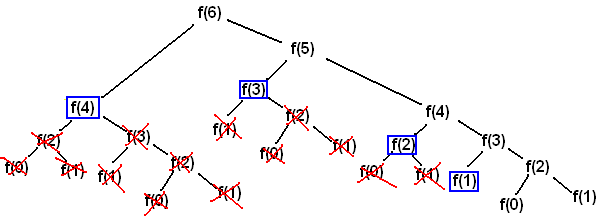
\includegraphics[scale=.4]{fibonacci_pd.png}
\end{center}

Dentro de este tipo de programación hay varios  algoritmos de implementación. Uno es el de top-down (por el significado en ingles de de arriba para abajo) o memoización y el otro bottom-up (por el significado en ingles de abajo hacia arriba), aunque existen bibliografías que consideran sólo a top-down como programación dinámica.
\\
En este análisis se implementarán de ambas formas de forma que se pueda ahondar más acerca de los beneficios de ambos. 
\bigskip
\subsubsection{Análisis}
\begin{verse}
La idea de un algoritmo que implemente {\it divide and conquer} y almacenamiento de subproblemas, sugiere empezar pensando este problema y dividiéndolo en problemas pequeños.\\
Se puede afirmar que la solución, si existe, puede dividirse en dos casos: la solución no contiene al primer elemento de C y entonces la solución resulte de formar V con la mínima cantidad de elementos de C': 
\[ C' = C - \{e_{1}\}\]
Y en particular debe ser óptima. Supongamos por el absurdo que no. La solución al problema sería K $\leq$ |C'|. Supongamos que existe un Q < K que es solución. Pero esto no puede pasar, porque por la propia definición de nuestra solución, se va a devolver la mínima cantidad de elementos, entonces no puede existir un valor menor de elementos que sea solución.
\\
La otra posible solución sería que $e_{1}$ sí sea parte de la solución, es decir, habría que encontrar elementos que sumen V' con los elementos del conjunto C' :
 \[ C' = C - \{e_{1}\}\]
\[ V' = V - e_{1}\]
O sea que la solución óptima sería 1 + K, K $\leq $ |C'|, K solución. Si existiese un Q $ $ < $ $1+K y la suma de los elementos de Q = V', es decir hay una solución mejor para el problema con C' y V'. Pero entonces ahora K = Q y la solución óptima es K + 1, donde el 1 representaría el primer $e_{1}$ que por el análisis de este caso formaba parte de la solución óptima.
\end{verse}

\bigskip
\subsubsection{Formulación recursiva}
Se define PD una función que recibe un conjunto S, de elementos enteros no negativos, un valor V entero no negativo y un entero que representa el tamaño de S inicial, devuelve el mínimo cardinal del subconjunto s perteneciente a S que todos los elementos suman V; si no existe se devuelve n, tamaño de S, simbolizando la imposibilidad de encontrar solución. \\
\[
\begin{array}{@{} r @{} c @{} l @{} }
&PD(S, V, n)&{}=\displaystyle
\begin{cases}
\ n &\text{si } \text |S| = 0 \wedge V \neq 0 
\\
\ 0 &\text{si } \text V = 0 
\\
PD($\{$e_{2},e_{3},\dots,e_{n}$\}$,V,n)  &\text{si } e_{1} $>$ V
\\
1 &\text{si } e_{1} $=$ V
\\
\min_{} (1 + PD($\{$e_{2},e_{3},\dots,e_{n}$\}$, V - e_{1}, n),PD($\{$e_{2},e_{3},\dots,e_{n}$\}$, V, ))&\text{otro caso }
\\
\end{cases}
\end{array}
\]


\subsubsection{Algoritmo Top Down}

\begin{codebox}
\Procname{$\proc{Topdown}(C,V, desde, memoria,n)$}
  \li \If $NoExiste(C,V,desde,memoria)$ \Then
  \li \If $desde < 0$ \Then
  	\li \If $V =0$ \Then 
  	\li $devolver:0$
  	\li \Else
  	\li $devolver:n$
  \End
  \End
\li \If $c_{desde}==V$ \Then
	\li	$Guardar(1,V,desde,memoria,n)$
	\li \Else
\li \If $C_{desde} > V$ \Then  
		\li $valor \gets Topdown(C,V,desde-1,memoria,n)$
		\li $Guardar(valor, V, desde, memoria,n)$
		\li \Else
		\li $valor1 \gets 1 + Topdown(C,V-C_{desde},desde-1,memoria,n)$
		\li $valor2 \gets Topdown(C,V,desde-1,memoria,n) $
		\li $valor3 \gets min(valor1,valor2)$ 
		\li $Guardar(valor3,V,desde,memoria,n)$	
  		\End
  \End
  \li $Devolver: -1$  $si$ $memoria_{desde,V} \geq n$
\li $Devolver: memoria_{desde,V}$ $si$ $no$

\end{codebox}

\begin{verse}
Esto asegura que cada problema que se quiera resolver primero verificará si no esta resuelto. Si lo está, accedemos a la información y la devolvemos. Si no está, se calcula, se guarda y se devuelve. Para tener un acceso eficiente, la implementación de memoria debe ser una matriz de |S| x V, donde $memoria_{desde,V}$ contiene la mínima cantidad de elementos que se necesitan para formar V con elementos de $C_{1}$ hasta $C_{desde}$. A nuestro algoritmo suponemos que llega ya iniciada, es decir, con -1 en todas las posiciones simbolizando que todavía no se guardo solución y en la posición (0,0) se completa con 0 como caso base. Desde es un dato bandera que se utiliza para saber desde dónde comenzar a buscar, porque el algoritmo parte de una problema que en caso de no tener solución pre-calculada se debe computar y es importante saber desde qué problema estamos se está haciendo esto. La primera vez que se llama la función desde = n, ya que hay que formar V con cualquier subconjunto de S. La ventaja de esta implementación con respecto a la próxima es que solo calcula los subproblemas que necesita y nunca calcula un subproblema más de una vez. Una de las desventajas es que al funcionar por recursión se almacena cada llamada recursiva y si la llamada genera un árbol muy grande podría aparecer un problema de memoria.\\
\end{verse}

\subsubsection{Código Fuente}
\begin{lstlisting}
int buscarValorObjetivoPD_top_down(vector<int> conj,  long long int valorObjetivo, int& sol,long long int &pasos) {
    sol=-1;
    if(conj.size() == 0){
        if(valorObjetivo == 0) {
            sol=0;
            return 0;
        }else{
            sol=-1;
            return -1;
        }
    }else if(valorObjetivo == 0) {
        sol=0;
        return 0;
    }
    vector<vector<int> > soluciones(conj.size(),vector<int>((valorObjetivo+1),-1)); //inicializo matriz n x V con -1
    soluciones[0][0]=0;
    sol=aux_top_down(conj,valorObjetivo,conj.size(),soluciones, conj.size()-1,pasos);
    (sol > conj.size() || sol == 0)? sol=-1 : 1;
    return sol;
}

int aux_top_down(vector<int> conjActual,  long long int valorObjetivo, int tamInicial, vector<vector<int> > & memoria, int desde,long long int &pasos) {
    pasos++;
    if(desde < 0) {
        if(valorObjetivo==0) {
            return 0;
        }else {
            return tamInicial+1;
        }
    }
    if(memoria[desde][valorObjetivo] == -1) { // si no esta calculada
        if(conjActual[desde] == valorObjetivo){
            memoria[desde][valorObjetivo] = 1;
        }else if(conjActual[desde] > valorObjetivo) {  //si el valor actual es mayor que el valor objetivo no puede ser parte de la sol
            memoria[desde][valorObjetivo] = aux_top_down(conjActual,valorObjetivo,tamInicial,memoria,desde-1,pasos);
        }else{
            memoria[desde][valorObjetivo] = min(1 + aux_top_down(conjActual,valorObjetivo-conjActual[desde],tamInicial,memoria,desde-1,pasos), aux_top_down(conjActual,valorObjetivo,tamInicial,memoria,desde-1,pasos));
        }
    }
    return memoria[desde][valorObjetivo];
}
\end{lstlisting}
\subsubsection{Algoritmo Bottom Up}
\begin{codebox}
\Procname{$\proc{BottomUp}(C,V,n)$}
\li $memoria \gets matriz$ $de$ $n$ $\cdot$ $V$ $de$ $enteros$ $vacia$
\li $cargarConValores(memoria,n)$
\li $memoria_{0,0} \gets 0$
\li \For $i \gets 2$ \To $n$
\li	 	\For $j \gets 1$ \To $V$
\li 		\If $C_{i} > j$ \Then
\li 			$memoria_{i,j} \gets memoria_{i-1,j}$
\li 	\Else
\li 			$valor1 \gets memoria_{i-1,j}$
\li 			$valor2 \gets 1 + memoria_{i-1,j-c_{j}} $
\li 			$memoria_{i,j} \gets min(valor1,valor2)$ 
		\End	
	\End  
\End
\li $Devolver: -1$  $si$ $memoria_{n,V} \geq n$
\li $Devolver: memoria_{n,V}$ $si$ $no$

\end{codebox}
\begin{verse}
A diferencia del algoritmo anterior donde a partir de un input se buscaba si estaba almacenada su solución y posteriormente si estaba se devolvía y si no se calculaba y devolvía, en este directamente a partir de un input, se computan todos los posibles subproblemas del input en una matriz de n $\cdot$ V y al final de todo se devuelve el problema inicial, es decir, se construyen todas las subsoluciones hasta llegar al problema grande y se devuelve su solución. En el algoritmo se puede ver los movimientos que hace por la matriz son: si el elemento en la posición i, C$_{i}$ es mayor que el valor objetivo, entonces la  solución va a venir de buscar en la fila anterior. Si en cambio esto no pasa, la solución también puede ser ir a la fila anterior o agregar el elemento c$_{i}$ a la solución y analizar ahora un nuevo problema, donde la busqueda de la solución será de la fila anterior pero con la columna movida hacia la izquierda, dado que cambió el valor objetivo. 
\\
La desventaja de esta implementación es que siempre se calculan todos los subproblemas, aunque como ventaja podría reducirse la complejidad espacial solo almacenando las filas que se vayan a utilizar, analizando cuál es el workflow dentro de las celdas de la matriz y eliminando las ya utilizadas.
\end{verse}

\subsubsection{Código Fuente}
\begin{lstlisting}
int buscarValorObjetivoPD_bottom_up( long long int &valorObjetivo, vector<int> &conj, int& sol,long long int &pasos) {
    sol = -1;
    if(conj.size() == 0){
        if(valorObjetivo == 0) {
            sol = 0;
            return 0;
        }else {
            sol = -1;
            return -1;
        }

    }else if(valorObjetivo == 0) {
        sol = 0;
        return 0;
    }
    vector<vector<int> > soluciones;
    soluciones.resize(conj.size()+1);
    for (int i = 0; i < conj.size()+1; ++i) {
        soluciones[i].resize(valorObjetivo+1);
    }
    vector<int> c = conj; //agrego un elemento a C para poder indexar de forma mas clara
    c.push_back(0);
    int aux = c[c.size()-1];
    c[c.size()-1] = c[0];
    c[0] = aux;
    for (int j = 0; j < valorObjetivo+1; ++j) {
        soluciones[0][j]=c.size();
    }
    soluciones[0][0]=0;
    for (int i = 1; i < c.size(); i++) {

        for (int j = 0; j < valorObjetivo+1; ++j) {
            pasos++;
            if(c[i] > j ) {//si el elemento actual supera el valor objetivo no puede ser solucion
                soluciones[i][j] = soluciones[i-1][j];
            }else {
                soluciones[i][j] = min((soluciones[i-1][j]),1+(soluciones[i-1][j-c[i]]));
            }
        }

    }
    sol = soluciones[c.size()-1][valorObjetivo];
    (sol > conj.size() || sol == 0)? sol=-1 : 1;
    return sol;
}
\end{lstlisting}


\subsubsection{Complejidad}
\begin{verse}
Podemos asegurar que la cantidad de operaciones del algoritmo nunca excederá n x V, que es la complejidad a la que estamos ajustados, dado que las operaciones en cada paso reducen al  valor objetivo actual o la cantidad de elementos con los que operar. Esto quiere decir que cada paso mueve nuestro {\it celda subproblema} empezando desde la última posición y moviéndose en cada paso una fila hacia arriba o columnas hacia la izquierda, hasta que el rango de la matriz no lo permite.
En el caso del bottom-up la complejidad en cualquier caso $\in$ O($n \cdot V$), mientras que en el top-down sólo la cota superior $\in$ O($n \cdot V$). 
\end{verse}

\section{Experimentación}
\begin{verse}
Las pruebas que se hagan con valores random se harán utilizando la libreria numpy en python y con diferentes distribuciones. Además, se testearán varias veces cada instancia en cada algoritmo para sacar un promedio de los tiempos de ejecución reduciéndo al mínimo las posibles oscilaciones circunstanciales.
\\
\subsection{Experimento 1}

Los primeros análisis sugiere empezarlos comparando los algoritmos más básicos como fuerza bruta y backtracking. Posiblemente el algoritmo de fuerza bruta no permita ser computado para tamaños de C excesivamente grandes y los otros algoritmos sí, entonces sería razonable que se experimenten los algoritmos de forma cruzada y estableciendo relaciones y no todos de forma simultánea porque podría perderse información.
Además, la implementación de los algoritmos sugiere que ante contextos de C pequeños, el crecimiento de ambos es similar hasta un determinado valor de n, mientras que para casos de C grandes fuerza bruta no sería opción. Veámoslo.
\\
Fijemos los valores de los elementos de C de forma aleatoria y acotados por n y al valor objetivo =$n^{3}$, asegurándonos con esto que las podas nunca van a funcionar, dado que nunca C sumará el valor objetivo y como no habrá solución tampoco se aplicará la poda por optimalidad. Esto significa que no conseguiremos exactamente un peor caso si no uno promedio, dado que estamos generando los elementos de forma random bajo determinados parámetros. Evaluemos para instancias de n = 1,2,$\cdots$26 que parecen ser instancias representativas del problema y dada la complejidad de fuerza bruta es posible con n superiores el tiempo de ejecución no sea razonable, de modo que para evitar la pérdida de información por falta de instancias para n más grandes lo vamos a reemplazar con más instancias. \\
\begin{center}
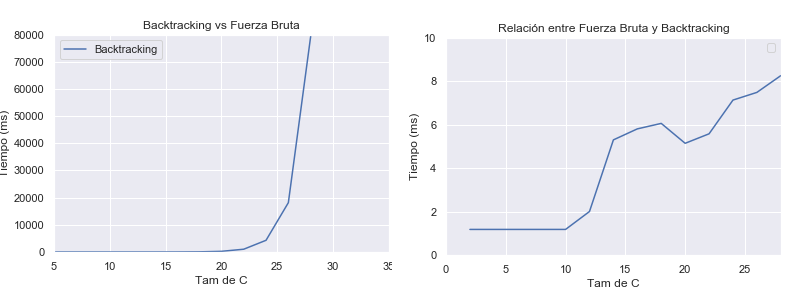
\includegraphics[scale=.4]{wc_bf_graph.png}
\end{center}
%\begin{center}
%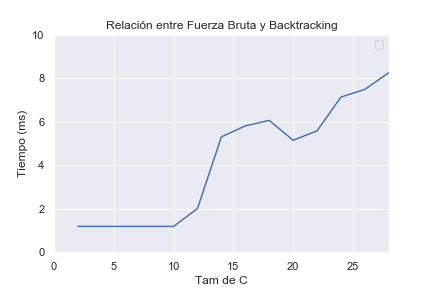
\includegraphics[scale=.4]{wc_rel_graph.png}
%\end{center}
Se puede ver la relación entre ambos algoritmos en función del tiempo. Por un lado, para contextos de tamaños de C chicos (hasta 20 elementos) los dos algoritmos tienen tiempos de ejecución similares, por eso se ve un tramo constante. Después hay crecimiento de fuerza bruta respecto de backtracking, lo cual coincide con el pensamiento inicial de que fuerza bruta es una solución {\it no tratable} como habíamos visto en la introducción. %Lo que se ve es una especie de inversión de crecimiento entre n = 18..22, pero hay que tener en cuenta que es muy puntual y representa un decrecimiento muy chico, está en función del tiempo en ms y básicamente es menos de un ms.\\
Veamos por último que efectivamente un gráfico del algoritmo de fuerza bruta demuestra que no sólo tiene un crecimiento exponencial sino que este ya es demasiado grande para n $\geq$ 25.
\\
Analicemos cuál es el resultados de utilizar algoritmos de programación dinámica en este tipo de instancias:
%\subsection{Experimento 2}
%Los algoritmos de programación dinámica si bien pertenecen a una misma caracterización, tienen implementaciones con rasgos que nos permiten pensar ciertas cosas: si tenemos un caso donde, por ejemplo, nuestro valor objetivo es de la misma magnitud que los elementos de C, quiere decir que en top-down rápidamente vamos a cómputar la solución, porque se reducen la cantidad de subproblemas (llamados recursivos) si los elementos de C son tan grandes como el valor objetivo, sin embargo, en bottom up de cualquier forma habría que computar todos los subproblemas. En el backtracking se activarían las podas y también se vería beneficiado. Aunque en un peor caso, si los valores de C son muy chicos, el recorrido de top down se va a extender demasiado y el backtracking actuaría como un fuerza bruta.\\
%Entonces iniciemos probando con n = 2 $\cdots$ 30, para tener una amplia gama de tamaños de C y lo suficientemente cercanos para ver los saltos, porque se supone que van a realizar los problemas más rápidamente y entonces necesitamos una mayor cantidad de instancias. Además, fijemos V aleatorio en el orden de $n^{3}$ para conseguir un espectro grande de valores y los elementos de C aleatorios en el orden de $n$. De esta forma nos tendremos una densidad uniforme entre los valores de C junto con un valor objetivo alto. Esperamos ver que el backtracking tenga un crecimiento asintótico al de fuerza bruta, que el top down a base de su memorización de resultados previos saque ventaja frente a bottom up, que a medida que n crezca tendrá matrices más grandes que completar.
\begin{center}
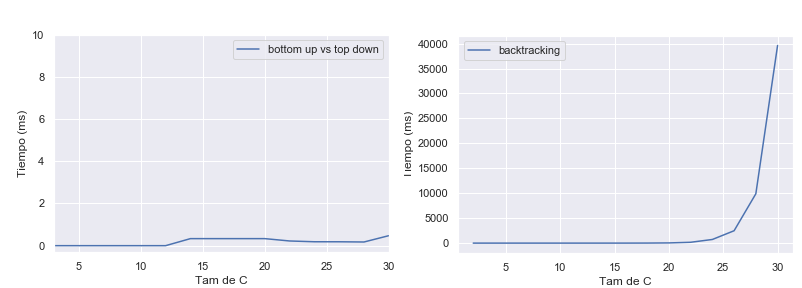
\includegraphics[scale=.4]{wc_bu_vs_td_graph.png}
\end{center}
Efectivamente los algoritmos de programación dinámica tienen tiempos similares en este tipo de instancias y el backtracking tuvo un comportamiento de crecimiento exponencial, aunque siendo ampliamente mejor ante un fuerza bruta.
%\begin{center}
%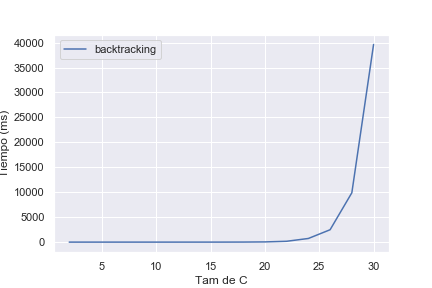
\includegraphics[scale=.4]{wc_bt_graph.png}
%\end{center}
Con este gráfico vemos cómo el backtracking en las instancias de peor caso (elementos de C de orden muy chico respecto a V)  y analizando una cantidad suficiente de instancias tiene un crecimiento exponencial como indica la complejidad teórica a la que pertenece.\\
Para terminar este análisis fijemos un n, los valores de C entre 0 y V y al valor objetivo entre n y $n^{3}$ para tener una gama amplio respecto de V. Veamos entonces más en profundidad si estas relaciones entre los algoritmos de programación dinámica realmente son por las relaciones entre V y elementos de C.\\
\begin{center}
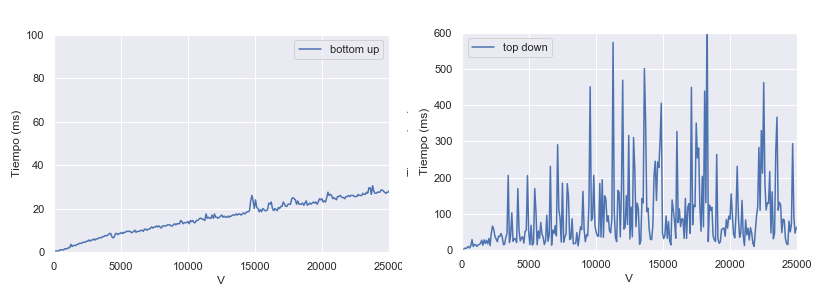
\includegraphics[scale=.4]{wc2_bu_vs_td_graph.png}
\end{center}
La razón de visualizar la información obtenida en gráficos separados es que ambos se mueven en diferentes escalas de tiempo, pero sin embargo hay hechos que se pueden resaltar. Ambos crecen a medida que V crece, aunque bottom up lo hace de forma mucho más estable que top down, que es parte de lo que queríamos probar. El motivo de las oscilaciones debe tener varias razones, intentemos explicar algunas: al determinar instancias tan grandes de datos se hace necesario generarlos aleatoriamente bajo determinados parámetros,  nada quita que la aleatoriedad genere casos borde que no pertenecerían a la media de instancias que buscamos generar. Por otro lado pero también afectado por esto, cuando existen instancias de tanta densidad de elementos de C acotados ampliamente por V, las llamadas recursivas de top down son cada vez más grandes y además no son gratis, hay que almacenarlas, si en particular una llamada genera un árbol de subproblemas excesivamente grande el problema es enorme.
\\
Un hecho curioso sacado de esto es que el backtracking, en este tipo de casos donde hay muchas chances de que las podas tengan una alta actividad, no solo compite sino mejora al bottom up como se ve a continuación:

\begin{center}
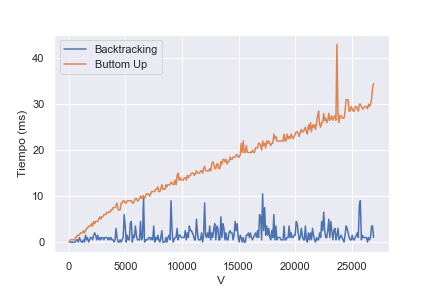
\includegraphics[scale=.4]{wc_bt_vs_bu_graph.png}\end{center}
%La explicación es simple: en estos casos particulares, backtracking actúa casi como un algoritmo lineal, porque son tantos los casos que evita calcular que es como si solo recorriera una vez a C, mientras que bottom up cada vez que V crece necesita matrices más grandes que recorrer.

\subsection{Experimento 2}
Ahora la cuestión es ver si existen instancias para las cuales convenga utilizar top-down en lugar de bottom up o backtracking. Para sacar ventaja frente a Bottom up necesitamos que n $\cdot$ V sea grande.
Para lo siguiente construimos intanicias incrementando n y V simultaneamente, y los elementos de C generamos aleatoriamente de forma uniforme acotados por V.\\
En el siguiente mapa de calor podemos ver de forma separada como es la relación de los tiempos de ejecución de cada algoritmo en función del tamaño de C y del valor objetivo. Como primer detalle vemos que las escalas de tiempo son diferentes: el top-down tiene gran parte de sus promedios de tiempos en los 5 segundos mientras que para el mismo tipo de instancias bottom up tiene promedios de 15. Por otro lado, vemos que en el bottom up los tiempos están más en función de n y V, es decir, es un algoritmo estable pero que se ve afectado por los tiempos que consume moverse en una matriz cada vez mas grande, a diferencia de top down. Este parece centraliza sus tiempos más grandes en una franja intermedia de los V. Por lo que venimos analizando, esto podría relacionarse con "peores" peores casos que al computarlos genera estas oscilaciones que venimos viendo, de modo que el top down ante casos en donde resuelve pocos subproblemas no se ve afectado por el n $\cdot$ V.
\begin{center}
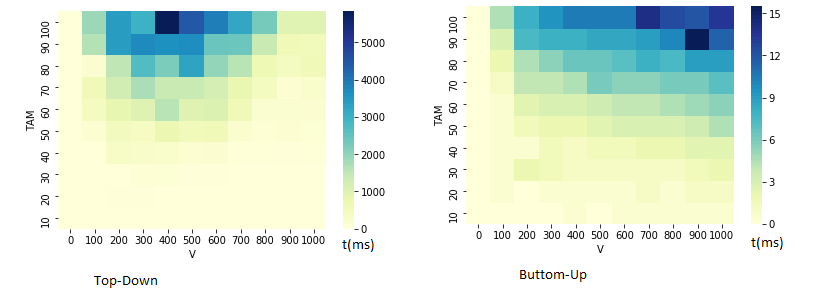
\includegraphics[scale=.4]{heatmap_td_vs_bu.png}
\end{center}
%Por último analicemos lo siguiente: Backtracking tiende a comportarse como lineal ante los casos en que V es de menor o igual orden que los elementos de C y bottom up demostró ser eficiente en ese tipo de instancias. La pregunta sería: si sabemos que estamos ante uno de estos contextos, cuál de los dos conviene?
%A simple viste se diría que backtracking, porque si es casi lineal claramente mejor que n x V. Sin embargo en nuestros análisis vimos que en los algoritmos recursivos las llamadas recursivas no son gratis y esto puede afectar la performance.
%\begin{center}
%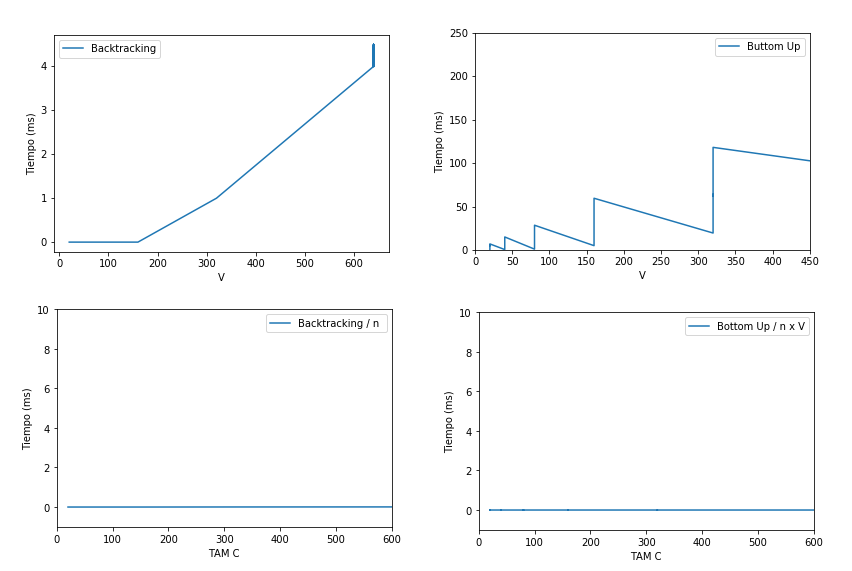
\includegraphics[scale=.4]{comp_bu_bt.png}
%\end{center}
\subsection{Experimento 3}
En la simulación de diferentes situaciones de la vida cotidiana se pueden utilizar distribuciones normales la generación de determinadas instancias. Sería interesante entonces analizar situaciones en las que los elementos estén generados de esta forma.
Analicemos la siguiente, fijemos n en 15,20,25, que nuestros experimentos arrojaron que eran valores razonables para probar simultáneamente los algoritmos: si los elementos de C siguen una distribución normal de media n, el valor objetivo lo hacemos incrementarse hasta $n^{3}$ y la varianza = $\frac{n^{2}}{V}$ inicialmente y después varianza = $\frac{V}{n}$. En el primer caso es una instancia en donde a medida que crece V, los elementos de C sufren una menor dispersión. Esto puede indicar que, en Backtracking mientras V no sea de un orden mucho mayor a n, como los elementos van a estar cerca de V las podas van a tener mucho trabajo y el algoritmo será eficiente. Por otro lado, si la dispersión se incrementa con V, Backtracking va a empeorar su performance debido a su reducción en el uso de las podas.\\
%En el caso de Fuerza Bruta no se esperan cambios, dado que no importa la situación siempre hará lo mismo. Para Top-Down y Bottom Up, no se esperan grandes beneficios, de hecho para Top-Down es posible que cuando la dispersión sea alta se le generen lamadas recursivas muy pesadas y (por la alta densidad de los elementos) y empeore su performance.\\
Se presentan los mapas de calor en función de V y n. En la parte superior están los gráficos cuando la dispersión disminuye cuando aumenta V.
\begin{center}
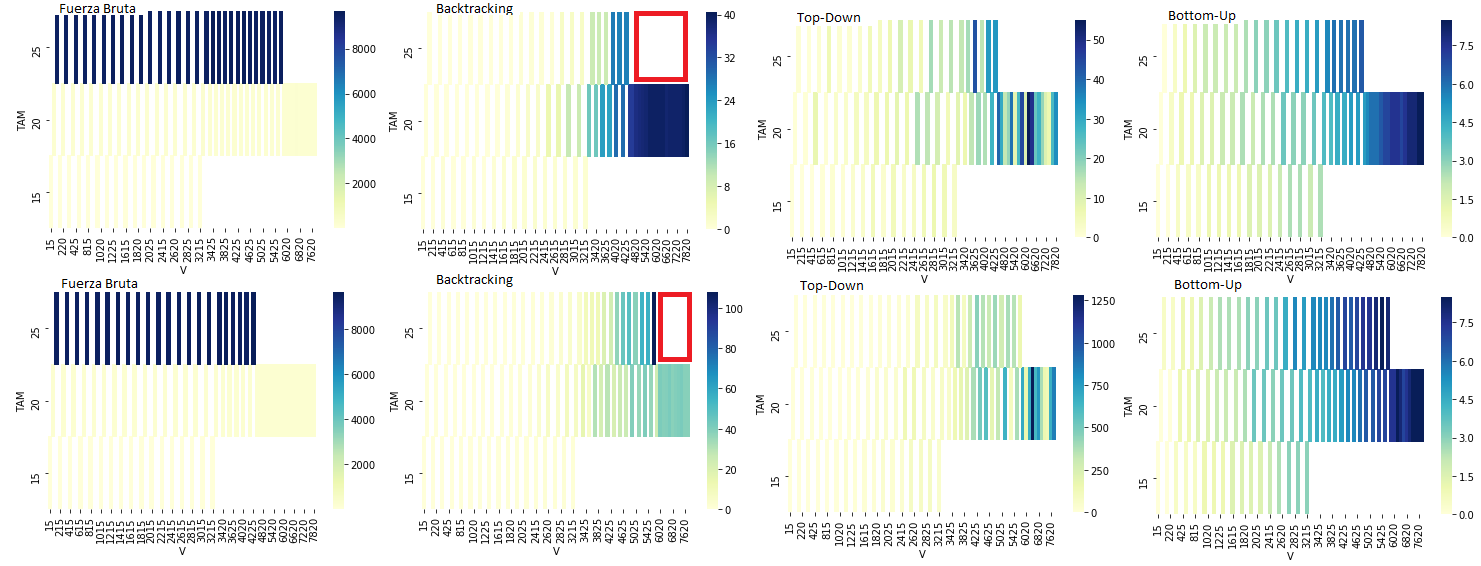
\includegraphics[scale=.4]{comp_distr_normal.png}
%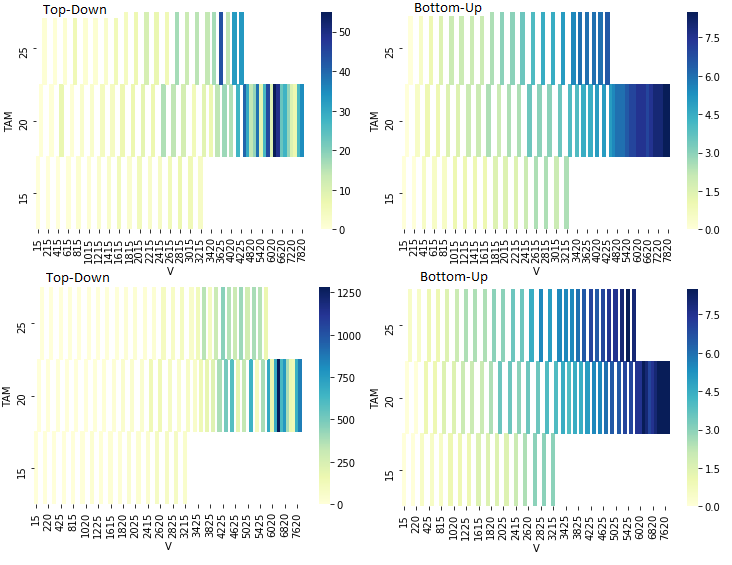
\includegraphics[scale=.5]{comp_distr_normal_2.png}
\end{center}
\end{verse}
Finalmente las ideas principales se puede apreciar que para Fuerza Bruta no hay cambios debido a que en cualquier caso realiza todos los subproblemas. Por otro lado Top-Down empeora considerablemente cuando la dispersión aumenta, aunque sorprende su alta eficiencia cuando es baja la dispersión. Lo que pasa es que no habíamos notado que Top-Down almacenará los resultados de los subproblemas y si esos subproblemas son muy parecidos (baja dispersión de los elementos) entonces se beneficiará mucho de esto, y esto evidentemente no se dará con una alta dispersión. \\
Respecto de Backtracking hubo ciertas diferencias. Posiblemente se deba a que el hecho de que haya o no dispersión lo afecta en tanto y cuanto los elementos no se alejen mucho de V, porque en ese caso casi que actuará con un Fuerza Bruta. Como nota: marcas rojas indican que por temás de tiempo de procesamiento no se llegaron a completar.

\section{Conclusiones}

\begin{verse}
%Durante la presentación de este trabajo se presentaron diferentes técnicas algorítmicas para hallar las soluciones del conocido problema {\it suma de subconjunos}. Cada una de estás técnicas responden a diferentes formas de abordar el problema para llegar a una solución. Inicialmente se hizo un análisis de la literatura del problema, mencionando diferentes algoritmos y sus objetivos principales. Posteriormente se escribieron cuatro diferentes algoritmos y desde ese momento se podían plantear interrogantes o afirmaciones acerca de qué tipo de situaciones o contextos podrían beneficiarlos. Finalmente se realizaron experimentos que permitieron conocer un poco más en profundidad los puntos débiles y fuertes de las soluciones, así como también adquirir la información suficiente a la hora de tomar decisiones de cuál de ellos experimentar en función del contexto, los recursos disponibles o las necesidades. \\
Los algoritmos que utilicen fuerza bruta quedan relegados para situaciones muy singulares, con tamaños de C muy pequeños, y su ventaja responde a la facilidad con la que se puede diseñar. Una mucho mejor opción se vio que era el Backtracking, no solo porque también es relativamente sencillo de diseñar sino porque permite ser útil en mayor variedad de situaciones. Vimos que si bien ante casos de C muy grandes padecía lo mismo que Fuerza Bruta, hay casos en lo que esto no pasa. Estos casos son cuando el orden de gran parte de los elementos de C supera al de V, porque vimos que el comportamiento en estas situaciones era casi lineal debido a la cantidad de combinaciones de soluciones que se salteaba.\\ 
Desde otro punto de la programación encontramos a Top-Down y Bottom up. La realidad en la experimentación es que Top-Down no fue tan beneficiado por los números, Bottom up demostró ser muy rápido para grandes muestras de tamaños de n y V, incluso los razonablemente grandes, y había que incrementarlos mucho para empezar a notar una deficiencia a base de los movimientos que debe hacer por la matriz. Incluso, en los mejores casos de Backtracking quedó ciertamente relegado para este tipo de casos, dado que al aumentar mucho n y V comenzaba a incrementar los tiempos, mientras que Backtracking al no tener este problema supo sacar las ventajas. \\
También es necesario mencionar que las facilidades para diseñar Bottom Up son propias de este problema y en otros podría ser realmente difícil, lo cual sumaría ventaja a Top-Down que es muy sencillo.\\
Como líneas finales queda resaltar la variedad con la que se puede intentar hacer frente a un problema, y lo importante de los análisis y experimentos que pueden trazar una ayuda acerca de los mejor pasos a seguir en situaciones determinadas. 

\end{verse}

\section{Referencias}
\begin{verse}
$[3]$Dynamic training subset selection for supervised learning in Genetic Programming, Chris GathercolePeter Ross.\\
$[4]$Generalizing Cryptosystems Based on the Subset Sum Problem, Aniket Kate and Ian Goldberg\\
$[5]$Thomas Cormen, Algorithms and Optimization, Approximation Algorithms, pág 1106\\
$[6]$G. J. Woeginger, Exact Algorithms for NP-Hard Problems: A Survey, Lecture Notesin Computer Science 2570, pp. 185-207  \\
$[7]$Computing partitions with applications to the knapsack problem,  Journal of the Association for Computing Machinery\\
$[8]$Donald Knuth. \it{The Art Of Computer Programming : Fundamentals Algorithms}
\end{verse}

\end{document}
